\documentclass[border=10pt]{standalone}
\usepackage{pgfplots}
\pgfplotsset{compat=1.18}
\begin{document}
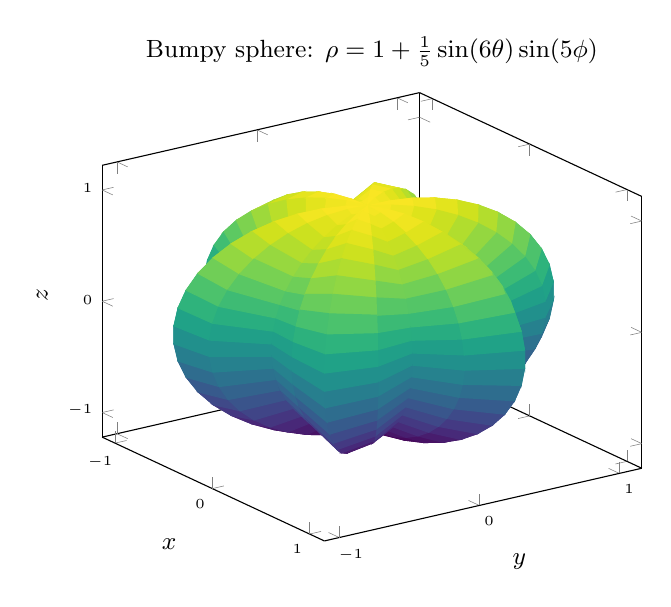
\begin{tikzpicture}
\begin{axis}[
    view={55}{25},
    domain=0:360, samples=24,
    y domain=0:180, samples y=24,
    z buffer=sort,
    colormap/viridis,
    xlabel={$x$}, ylabel={$y$}, zlabel={$z$},
    title={Bumpy sphere: $\rho = 1 + \frac{1}{5}\sin(6\theta)\sin(5\phi)$},
    tick label style={font=\tiny},
    label style={font=\small},
    title style={font=\small},
]
\addplot3[surf, shader=flat]
(
 {(1 + 0.2*sin(6*x)*sin(y))*sin(y)*cos(x)},
 {(1 + 0.2*sin(6*x)*sin(y))*sin(y)*sin(x)},
 {(1 + 0.2*sin(6*x)*sin(y))*cos(y)}
);
\end{axis}
\end{tikzpicture}
\end{document}
